\chapter{Question 2}
\label{avoiding-uri-aliases} 

\textbf {Take the Twitter graph you generated in question 1 and test for male-female homophily.  For the purposes of this question you can consider the graph as undirected (i.e., no distinction between ``follows'' and ``following'').  Use the twitter name (not ``screen name''; for example ``Michael L. Nelson'' and not ``@phonedude\textunderscore mln'') and programatically determine if the user is male or female.  Some sites that might be useful:}\\
\url{https://genderize.io/}\\
\url{https://pypi.python.org/pypi/gender-detector/0.0.4}\\
\textbf {Create a table of Twitter users and their likely gender.  List any accounts that can't be determined and remove them from the graph.
}\\
\textbf{Perform the homophily test as described in slides 11-15, Week 7.}\\
\textbf{Does your Twitter graph exhibit gender homophily?}

Following are the steps I have taken to solve the problem:
\begin{itemize}
\item I split the names of each follower into last name, first name and initial. 
\item By considering the first name of each user I found the gender of each follower using genderize API.
\item I updated the JSON data in question 1 by adding gender to each follower.
\newpage
\item The screen shot of updated JSON data is in Figure \ref{fig:q1fig1}
\begin{figure}[h!]
\begin{center}
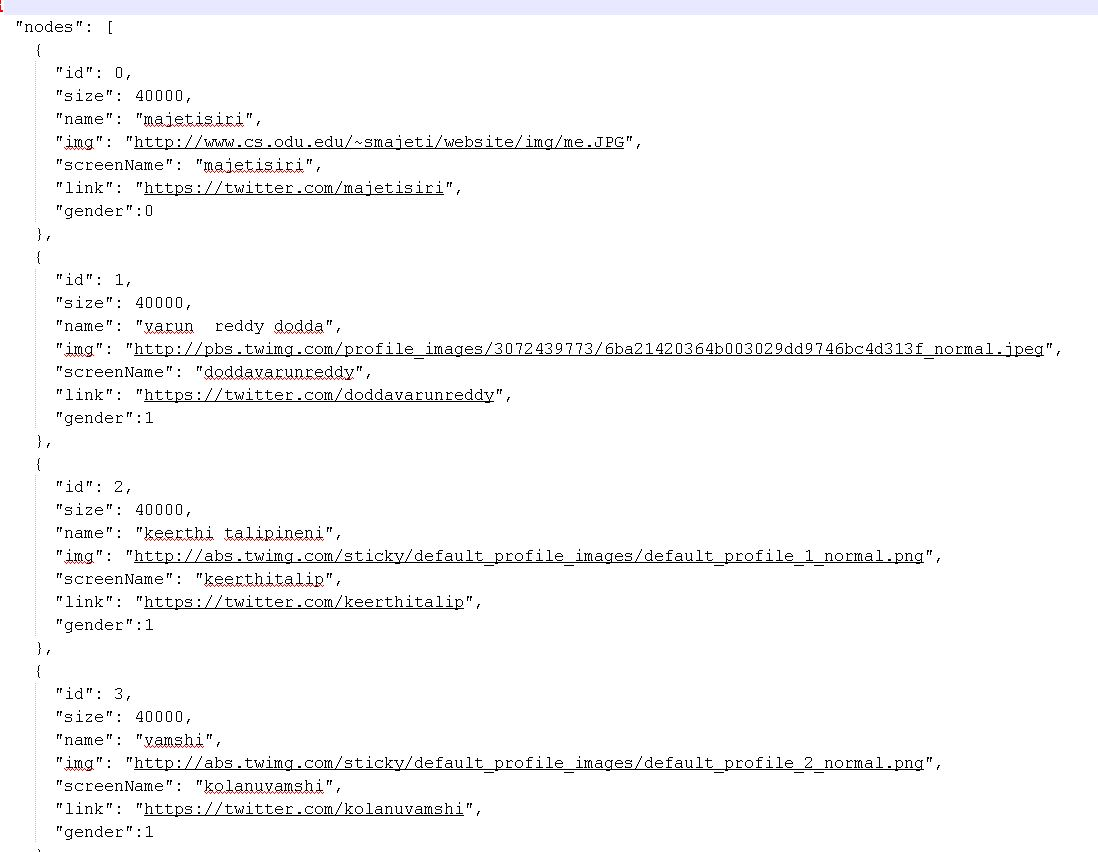
\includegraphics[scale=0.55, keepaspectratio=true]{figures/6.JPG}
\caption{Output of updated nodes data}
\label{fig:q1fig1}
\end{center}
\end{figure}
\item The code is listed in Listing \ref{lst:q2code1}.
\newpage
\item This data is taken as input for D3 to generate a graph which differentiates the followers based on gender. 
\item The table with list of followers and their gender is illustrated in Table \ref{Table:q1table1}. 
\begin{table}

\caption{Table with followers and gender}
\label{Table:q1table1}
\begin{center}
\begin{tabular}{| c | c |}
\hline

 Name | Gender\\ \hline
 Naina  | female\\ \hline		
 veena  | female\\ \hline		
 Shivani| female\\ \hline		
 Sneha  | female\\ \hline		
 erika  | female\\ \hline
 Mayra  | female\\ \hline	
 Ivy    | female\\ \hline
 Marion | female\\ \hline
 Mamie  | female\\ \hline	
 Augusta| female\\ \hline
 Lauri  | female\\ \hline	
 Ashlee | female\\ \hline
 Sadie  | female\\ \hline	
 Angie  | female\\ \hline
 Sophia | female\\ \hline
 Myrtle | female\\ \hline	
 Trisha | female\\ \hline
 Lara   | female\\ \hline	
 Sandra | female\\ \hline
 Tammi  | female\\ \hline	
 Divya  | female\\ \hline
 deepa  | female\\ \hline
 sudha  | female\\ \hline
varun| 		male\\ \hline		
keerthi|	male\\ \hline		
vamshi| 	male\\ \hline		
srinivas|	male\\ \hline		
sai| 		male\\ \hline
Jesse|		male\\ \hline	
Prasanna| 	male\\ \hline
Nishant`| 	male\\ \hline
Ravi| 		male\\ \hline	
manoj| 		male\\ \hline
Eric| 		male\\ \hline	
Masroor| 	male\\ \hline
Rahul| 		male\\ \hline	
Adrian|		male\\ \hline
vinay| 		male\\ \hline
dinesh| 	male\\ \hline
BhavaniManthena	|	null\\ \hline		
Mounica		|		null\\ \hline		
Vam				|	null\\ \hline		
Mounica|			null\\ \hline		
KatherineEdmunds|	null\\ \hline
Basani			|	null\\ \hline	
Deepthikrovi| 		null\\ \hline
rajyalakshmi| 		null\\ \hline
Rithika		|		null\\ \hline	
Doomie		|		null\\ \hline
satvikgadam   |  	null\\ \hline	
                
\end{tabular}
\end{center}
\end{table}
\item There are 11 followers whose gender is `null'. When I tried to get my gender with my first name `majetisiri' it gave a `null'. If I draw a graph by removing nodes with `null' gender, it leads to removal of 80 percentage of the links in the graph. So I created a graph including followers who have a `null' gender.
\item All male followers are represented in color `orange', female followers in color `green' and those whose gender is not determined are represented in color `blue'. This graph is illustrated in Fgure \ref{fig:q1fig2}
\newpage
\item Yes, the graph exhibits gender homophily. Most of the female followers are followed by or following female users. As the graph generated is a force directed graph if we pull a node in `green', we can see all the `green' nodes connected to it.
\begin{figure}[h!]
\begin{center}
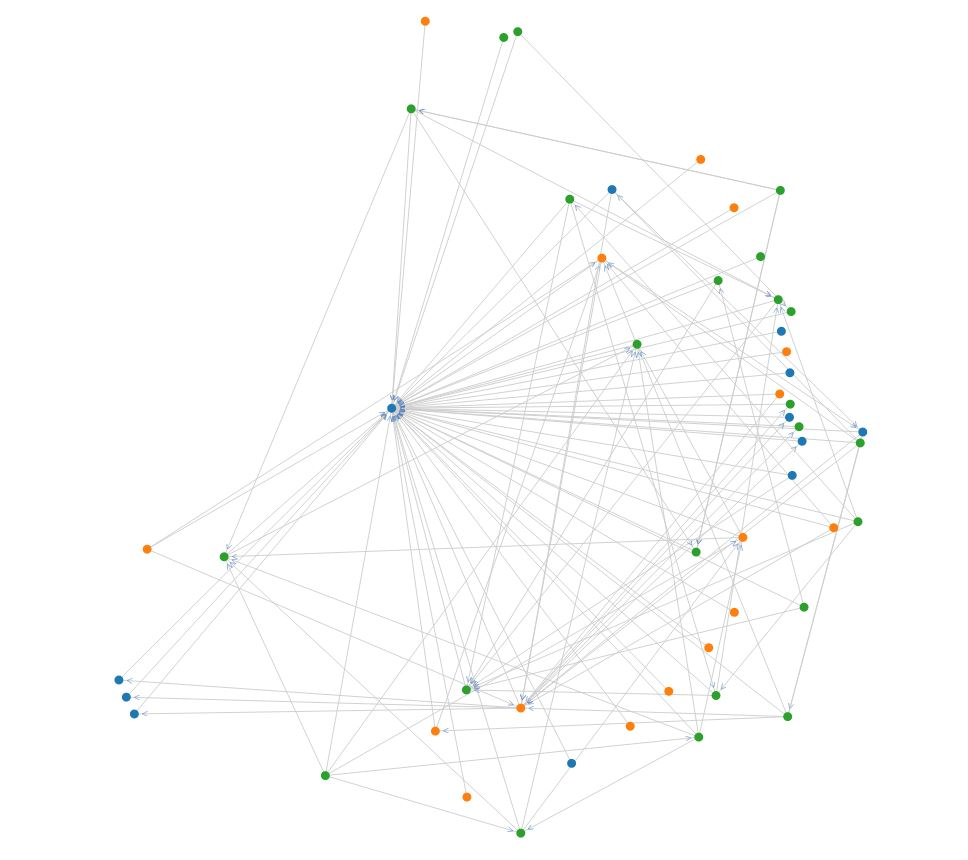
\includegraphics[scale=0.55, keepaspectratio=true]{figures/5.JPG}
\caption{Output Graph with followers distinguished based on gender}
\label{fig:q1fig2}
\end{center}
\end{figure}
\item This graph is located at URI \url{http://bl.ocks.org/majetisiri/fd87d5725027a5441f78}
\end{itemize}

\newpage
\textbf{Code Listing}
\sloppy
\lstinputlisting[language=Python,caption=Python code for getting gender for followers using their first name,frame=single,breaklines=true,label=lst:q2code1, tabsize=2, captionpos=b,numbers=left,showspaces=false,showstringspaces=false,basicstyle=\footnotesize]{src/gender.py}



